\section{Setting up a CockroachDB Cluster with Docker}\label{chap:how-to}
\emph{author: Felix Tröbinger}\bigskip

\subsection{Creating a bridge network}
Even though all created nodes -- or rather containers -- in this example will run on the same host, they still need to be connected via a network of some sorts. As a solution this example will use a Docker \emph{bridge network}.

A bridge network is a software bridge, which allows containers on the same host to communicate with each other. Features of docker bridge networks are that user-defined bridges provide automatic DNS resolution between containers and that containers are isolated in a better way.\cite{docker-bridge}

\medskip
The following command will create a bridge network called \verb|roachnet|. This name will be passed to each node on startup/creation.

\begin{verbatim}
docker network create -d bridge roachnet
\end{verbatim}

\subsection{Creating Nodes}\label{chap:creating-nodes}

This example will create a cluster of three connected nodes. The first one is created with the following command.

\begin{verbatim}
docker run -d \
--name=roach1 \
--hostname=roach1 \
--net=roachnet \
-p 26257:26257 -p 8080:8080  \
-v "${PWD}/roach1:/cockroach/cockroach-data"  \
cockroachdb/cockroach:latest start \
--insecure \
--join=roach1,roach2,roach3
\end{verbatim}

The node is connected to the previously created bridge network and given a name, \verb|roach1| in this case.

\medskip
Port 8080 of the host machine is mapped to port 8080 of the container which is later used for accessing the web-interface (See chapter \ref{chap:web-interface}).
Port 26257 of the container is mapped to the same port on the host. This port is used for communication.

\medskip
Adding a volume to the container will give the user the possibility to see what CockroachDB stores on disk and save data on container restart. To completely reset the node, the user has to delete the volume. If no volume is mapped on container start, all data will be lost when the container stops. 

\medskip
The Docker image in use is called \verb|cockroachdb/cockroach| and this example uses the latest version. The command \verb|start| is passed, which will start the CockroachDB inside the container.

\medskip
For the time being this example will use the insecure mode of CockroachDB which does not require certificates. More on that in chapter \ref{chap:secure}. 

\medskip
Finally the command will use the \verb|join| argument to connect the three nodes in the cluster by specifying their \verb|hostname|.

\bigskip
For this example two more nodes will be created (nodes \verb|roach2| and \verb|roach3|) using a very similar command as the one above, only changing the hostname and the volume directory on the host machine. The last thing that differs for the last two nodes is that the ports will not be mapped as witch \verb|roach1|. This is because when the web-interface in this example will be accessed, it will access the first created node. For more information about the web-interface see chapter \ref{chap:web-interface}.
\bigskip

As the next step the cluster has to be initialized. This is done with the following command:

\begin{verb}
docker exec -it roach1 ./cockroach init --insecure
\end{verb}

\cite{cockroachdocker}

\subsection{SQL Command Line}
Using the CockroachDBs SQL client can be done via the following command. In this example the SQL client is used by accessing the first node that was created, \verb|roach1|.
\begin{verbatim}
docker exec -it roach1 ./cockroach sql --insecure
\end{verbatim}

CockroachDB uses the \emph{PostgreSQL} dialect.

\subsection{Web-Interface}\label{chap:web-interface}
Accessing the admin web-interface user interface is as easy as navigating to \verb|localhost:8080| in a browser. Port 8080 is used because the host port 8080 is mapped to port 8080 on \verb|roach1|. If this is already in use by another application running on the host machine, port 8080 within the container can be remapped to a different port on the host machine. This would be done by changing \verb|-p 8080:8080| to \verb|-p <YOUR-PORT>:8080| in the command that started the first node.

\begin{figure}[H]
    \caption{Cluster Overview}
    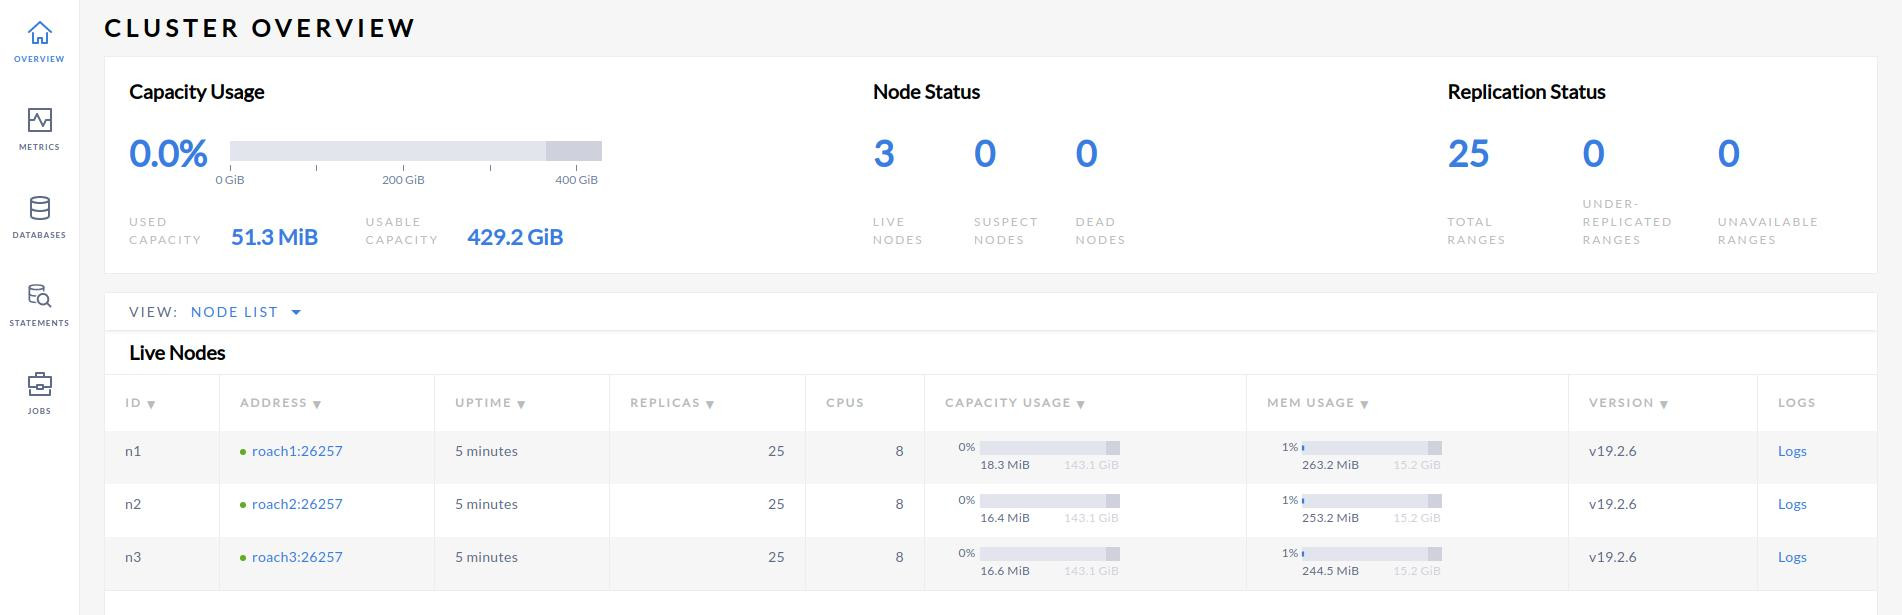
\includegraphics[width=\textwidth]{overview}
    \label{fig:overview}
\end{figure}

The first view the user is greeted with is the overview of the cluster which can be seen in Figure \ref{fig:overview}. This view shows all nodes connected to the cluster and the cluster capacity as well as the capacities for every single node.
Also visible is the amount of failing and failed nodes. In the \emph{Replication Status} one can see how many ranges/cells are stored and replicated across all CockroachDB nodes. 

\medskip
In the above figure, the three previously created nodes are visible and all running. Note that every node thinks its full capacity regarding disk and memory usage are that of the main host. So in this case all three nodes assume that they can use the entirety of remaining disk space and RAM even though they really have to share these resources with the rest of the CockroachDB nodes (or really any other container or service) that also happens to run on the host machine.  

\medskip
Clicking on the \emph{Logs} button next to the node in the \emph{Live nodes} view would allow the user to see Logs specific for each node. In this example this is unavailable because the debugging mode is set to \verb|local| by default which disables this feature.

\begin{figure}[H]
    \centering
    \caption{The CockroachDB Web-Interface Dashboard}
    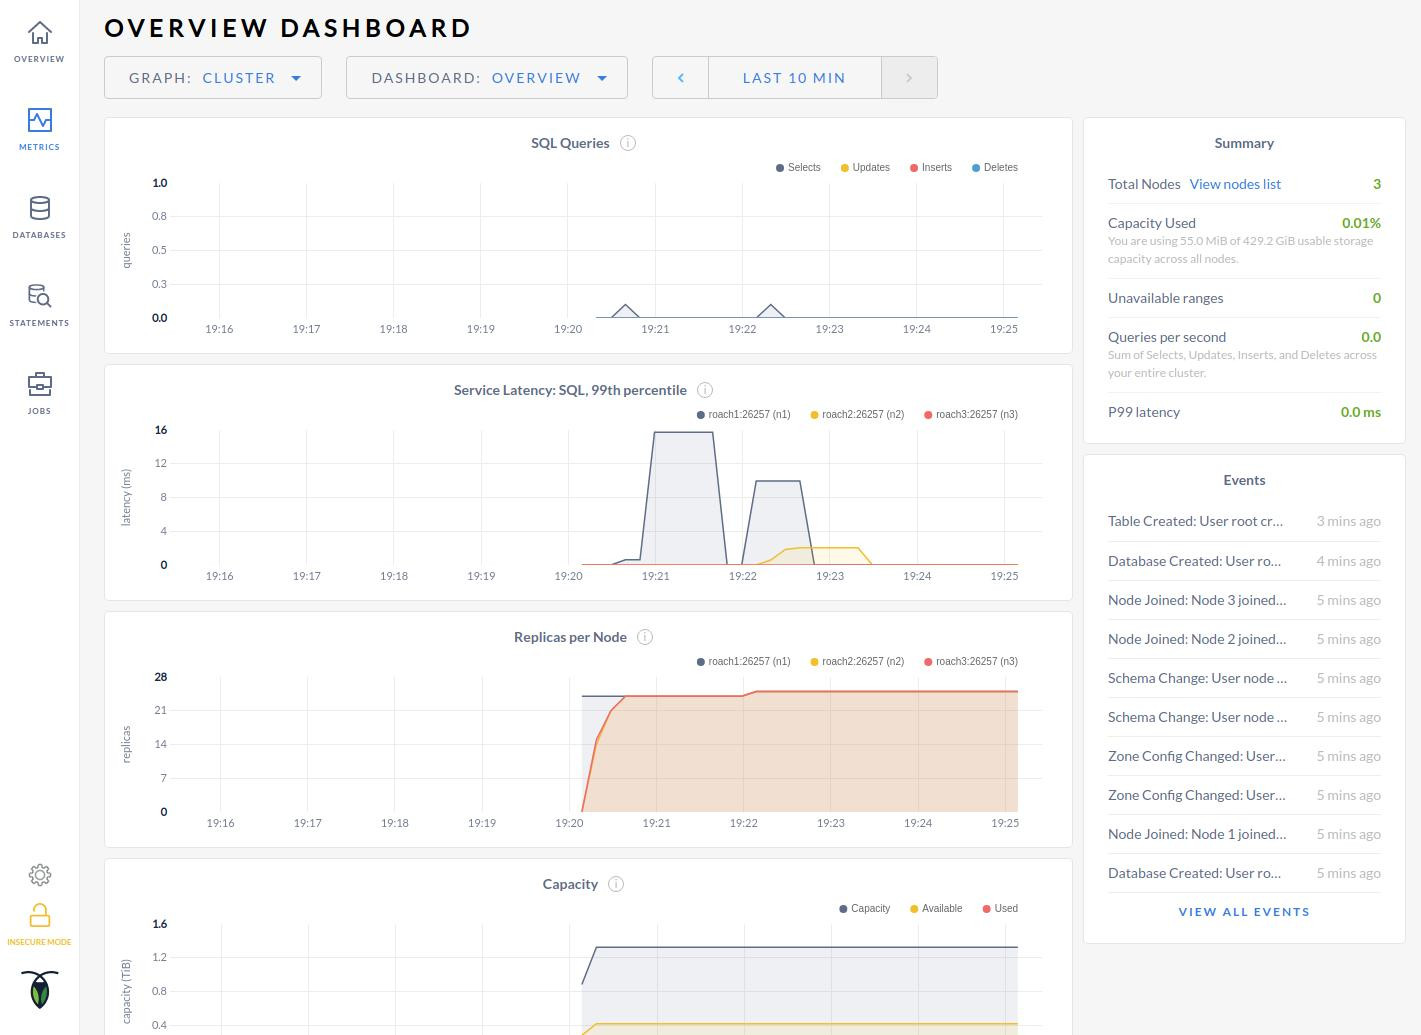
\includegraphics[width=\textwidth]{dashboard}
    \label{fig:dashboard}
\end{figure}

On the Dashboard view (also labeled \emph{Metrics} in the web UI) users can see graphs of SQL Queries ran on different nodes as well as latency and replication information.
In this example we created tables and inserted data on the first node. This is visible in the \emph{Replicas per node} graph where the line representing \verb|roach1| immediately jumps to the value whereas the other two nodes take a little bit of time replicating the data on their system. 

On the right-hand side a list of events that occurred in the database system is visible. In the example you can see that the latest events were the creation of the database and the tables therein.

\begin{figure}[H]
    \caption{View of databases}
    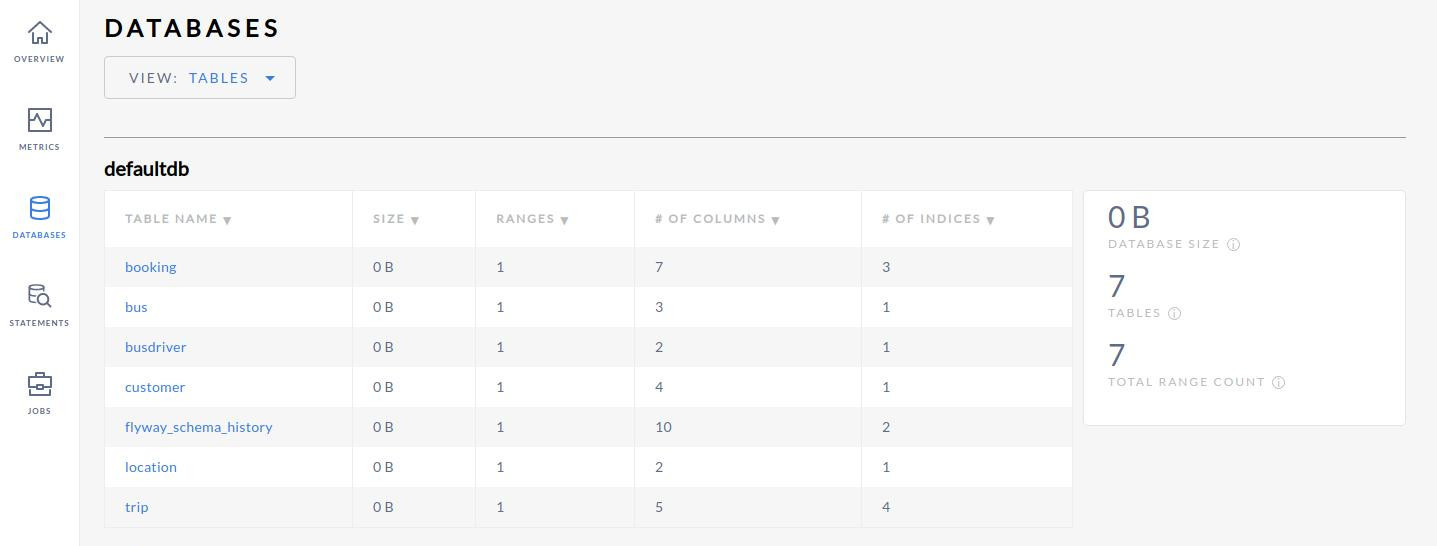
\includegraphics[width=\textwidth]{databases}
    \label{fig:databases}
\end{figure}
The \emph{Databases} view show a list of all databases and lists their tables. Note that it does not display contents of the database.

\begin{figure}[H]
    \caption{View of statements}
    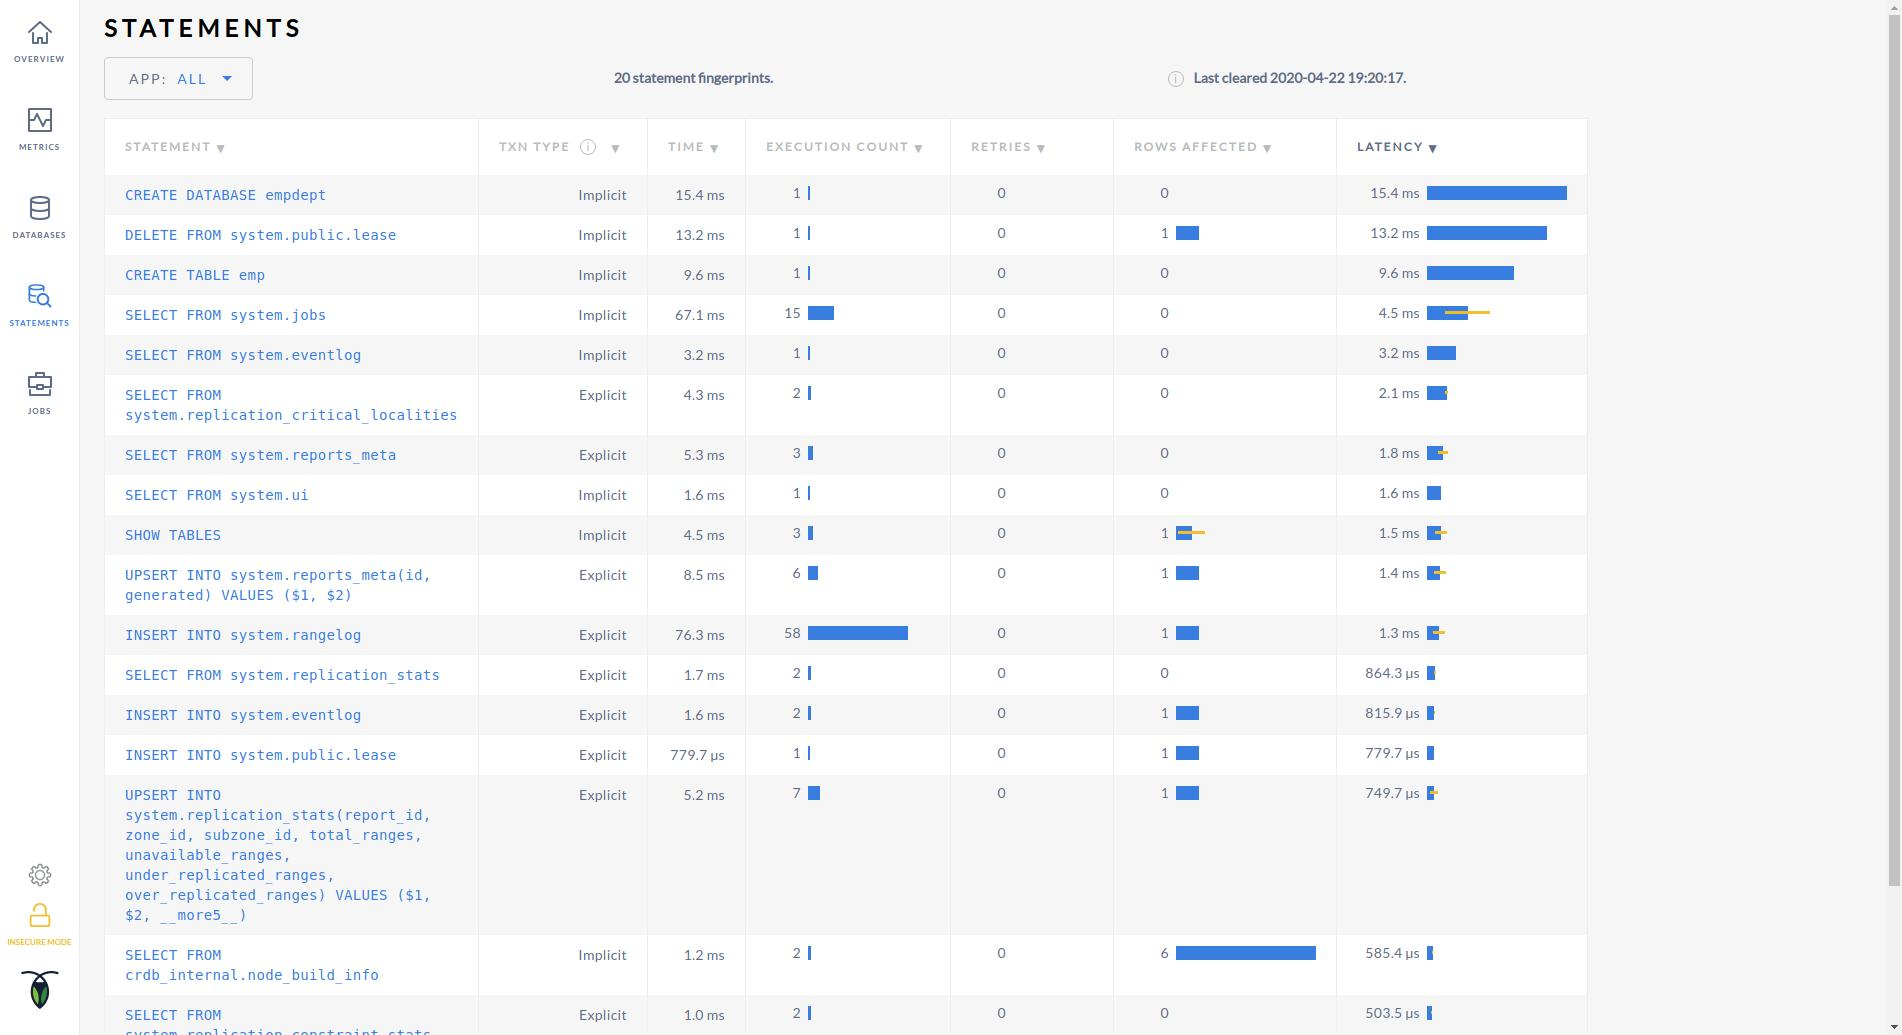
\includegraphics[width=\textwidth]{statements}
    \label{fig:statements}
\end{figure}

The \emph{Statements} view list all executed SQL commands/statements which can be filtered and sorted. 

\subsection{Securing the Cluster}\label{chap:secure}
\emph{author: Felix Tröbinger}\bigskip

In the previous example all nodes have been started with the command line option \verb|--insecure|. In the bottom of the web-interface the user is also reminded that CockroachDB is running in insecure mode by the golden lock icon. This is obviously a bad idea to be used in production or for any database, really. 

\medskip
Running CockroachDB in secure mode requires using certificates. These can be created by running either the \verb|cockroach cert| command or using \verb|opensll|. Alternatively a custom CA can be used.\cite{cockroach-cert}
For this example the Cockroach command will be used.

\begin{verbatim}
cockroach cert create-ca \ 
    --certs-dir=certs \
    --ca-key=my-safe-directory/ca.key
\end{verbatim}

The above command generates 
\begin{enumerate}
    \item a CA (= \textbf{C}ertificate \textbf{A}uthority) certificate and clients/node certificates
    \item a CA key 
\end{enumerate}

When creating secure nodes or client certificates the CA key is required and referenced during the creation process.
In a scenario where the CA key is lost, adding nodes to a cluster created from nodes that were signed with keys is not possible anymore.

\medskip
Creating certificates and key pairs for a node can be done with the following command. (Replace \emph{hostname} with your hostname/container name.)

\begin{verbatim}
cockroach cert create-node \ 
    localhost $(hostname) \
    --certs-dir=certs \
    --ca-key=my-safe-directory/ca.key
\end{verbatim}

When using a Docker container the certificates have to be in a specific directory of the container.
When starting the container the \verb|--certs-dir| is used to tell the container the specified location of the certificates. Similarly the \verb|--ca-key| option is used to tell the container the location of the CA key when creating it.
One possibility to add the certificates to the container is to use the volume command-line-parameter (similar to the one that was used to create nodes in the beginning of chapter \ref{chap:creating-nodes}.
A perhaps more elegant solution would be a Dockerfile that specifies options for either a single node or an entire cluster of nodes that run on a single machine.

The command will use the CA key that was created in the first command and stored in the \emph{my-safe-directory} directory to create certificates for the new node.

\bigskip
In the next step a certified client is created, in this case for a user called \emph{fred}.

\begin{verbatim}
cockroach cert create-client fred \ 
    --certs-dir=certs \
    --ca-key=my-safe-directory/ca.key
\end{verbatim}

After this step a SQL user by the same name is created and granted some rights in the database.
\cite{cockroach-security}

\begin{verbatim}
cockroach sql \
    --certs-dir=certs \
    --host=localhost:26257 \
    --execute="CREATE USER fred;
    GRANT SELECT ON TABLE db.example_table TO fred;"
\end{verbatim}

A certified client can then be used in an application.
